%%%%%%%%%%%%%%%%%%%%%%%%%%%%%% -*- Mode: Latex -*- %%%%%%%%%%%%%%%%%%%%%%%%%%%%
%% diss-related.tex -- 
%% Author          : Carleton Moore
%% Created On      : Thu Sep  2 11:02:52 1999
%% Last Modified By: Carleton Moore
%% Last Modified On: Wed Oct 27 10:29:35 1999
%% RCS: $Id: diss-related.tex,v 1.3 1999/10/27 20:29:41 cmoore Exp $
%%%%%%%%%%%%%%%%%%%%%%%%%%%%%%%%%%%%%%%%%%%%%%%%%%%%%%%%%%%%%%%%%%%%%%%%%%%%%%%
%%   Copyright (C) 1999 Carleton Moore
%%%%%%%%%%%%%%%%%%%%%%%%%%%%%%%%%%%%%%%%%%%%%%%%%%%%%%%%%%%%%%%%%%%%%%%%%%%%%%%
%% 

\chapter{Related Work}
\label{sec:related}

\begin{quote}
{\em If you don't know what you are doing, it is hard to improve it.} -- Watts Humphrey
\end{quote}

LEAP is a result of our experience using the Personal Software Process (PSP)
for over three years, our experience with Formal Technical Review (FTR) and our
attempts to improve the quality of software development.  This chapter briefly
discusses the PSP, some of the different tools developed to support the PSP,
and the software quality assurance process called Formal Technical Review.  The
chapter concludes with a discussion of measurement dysfunction and some of the
data quality issues found in the PSP and FTR.

\section{Personal Software Process}

The Personal Software Process\cite{Humphrey95} is a self-improvement process
for software developers. In his book ``A Discipline for Software Engineering''
Watts Humphrey teaches software developers how to become their own software
development coaches. Sports coaches observe the performance of their players,
evaluate their performance, then make suggestions for improvement.  This is the
classic {\em observe, evaluate, modify} cycle for improvement.  Software
developers using the PSP can become their own coaches.  The developer records
how they develop software and after each project they self-evaluate how they
performed.  These evaluations should lead to improvements on future projects.
In other words, The software developer conducts a longitudinal case study of
their own development process.  They can initiate changes and observe the
effects of those changes.

\subsection{Goals}
Two main goals of the PSP are \begin{itemize}
\item{to produce high-quality software as efficiently as possible and}
\item{to improve the developers ability to estimate the amount of effort required 
to produce the software.}
\end{itemize}
These two goals drive the whole PSP. The data collection and analyses are
focused on improving the developer's software development and estimation
skills. 

\subsection{Learning the PSP}

To teach developers how to use the PSP, Humphrey defines seven PSP processes (0,
0.1, 1.0, 1.1, 2.0, 2.1, 3.0). Each process has detailed scripts telling the
user exactly how to perform the process. Figure \ref{fig:psp-levels} shows the
seven levels.  Exercises at the end of each chapter in ``A Discipline for
Software Engineering'' ask the reader to use the knowledge from the chapter to
improve their development skills. The chapters introduce powerful development
techniques: design and code reviews, size and time estimation methods, and
design templates. These techniques help the developer produce high quality
products efficiently.  As developers go through the book they develop 10 small
software projects using the different PSP levels.
\begin{center}
  \begin{figure}[htb]
    \setlength{\unitlength}{2.5cm}
    \begin{picture}(5,5)
      \put(0,0.4){\parbox[b]{2.0cm}{Baseline Personal Process}}
      \put(0.75,0.25){\framebox(1.25,0.75){\parbox[b]{2.5cm}{{\bf PSP0} Time
            \& Defect recording}}}
      \put(2.0,0.35){\framebox(1.25,0.75){\parbox[b]{2.5cm}{{\bf PSP0.1} Coding
            Standard, Size Measurement}}}
      \thicklines
      \put(1.5,1.25){\oval(1.0,1.0)[tl]}
      \put(1.5,1.75){\vector(1,0){0.2}}
      \thinlines
      \put(0.5,1.4){\parbox[b]{2.0cm}{Personal Planning Process}}
      \put(1.75,1.25){\framebox(1.25,0.75){\parbox[b]{2.5cm}{{\bf PSP1} Size
            \& Time estimation}}}
      \put(3.0,1.35){\framebox(1.25,0.75){\parbox[b]{2.5cm}{{\bf PSP1.1} Task
      \& Schedule Planning}}}
      \thicklines
      \put(2.5,2.25){\oval(1.0,1.0)[tl]}
      \put(2.25,2.75){\vector(1,0){0.2}}
      \thinlines
      \put(1.0,2.4){\parbox[b]{2.2cm}{Personal Quality Management}}
      \put(2.75,2.25){\framebox(1.25,0.75){\parbox[b]{2.5cm}{{\bf PSP2} Code \&
      Design Reviews}}}
      \put(4.0,2.35){\framebox(1.25,0.75){\parbox[b]{2.5cm}{{\bf PSP2.1} Design 
      Templates}}}
      \thicklines
      \put(3.5,3.25){\oval(1.0,1.0)[tl]}
      \put(3.5,3.75){\vector(1,0){0.2}}
      \thinlines
      \put(1.5,3.4){\parbox[b]{2.0cm}{Cyclic Personal Process}}
      \put(3.75,3.25){\framebox(1.25,0.75){\parbox[b]{2.5cm}{{\bf PSP3} Cyclic Development}}}
    \end{picture}
    \caption{PSP levels}
    \label{fig:psp-levels}
  \end{figure}
\end{center}

\subsubsection{PSP0: The Baseline Process}

The baseline processes PSP0 and PSP0.1 introduce the concepts of data
collection and size measurement to the developer. The purpose of these
processes is to give the developer a basis for their improvement.  The
developer learns exactly how they develop software.  They learn to use the Time
Recording Log, Defect Recording Log and Postmortem forms to record and analyze
time, size and defect data.  In these two processes the developer uses the
planning, design, code, compile, test and postmortem phases. Figure
\ref{fig:psp01-phases} shows the order of the phases.
\begin{center}
  \begin{figure}[htb]
    \setlength{\unitlength}{2.5cm}
    \begin{picture}(6,1)
      \put(0,0.25){\framebox(0.75,0.5){Planning}}
      \thicklines
      \put(0.75,0.5){\vector(1,0){0.25}}
      \thinlines
      \put(1,0.25){\framebox(0.75,0.5){Design}}
      \thicklines
      \put(1.75,0.5){\vector(1,0){0.25}}
      \thinlines
      \put(2,0.25){\framebox(0.75,0.5){Code}}
      \thicklines
      \put(2.75,0.5){\vector(1,0){0.25}}
      \thinlines
      \put(3,0.25){\framebox(0.75,0.5){Compile}}
      \thicklines
      \put(3.75,0.5){\vector(1,0){0.25}}
      \thinlines
      \put(4,0.25){\framebox(0.75,0.5){Test}}
      \thicklines
      \put(4.75,0.5){\vector(1,0){0.25}}
      \thinlines
      \put(5,0.25){\framebox(0.75,0.5){Postmortem}}
    \end{picture}
    \caption{PSP0.1 phases}
    \label{fig:psp01-phases}
  \end{figure}
\end{center}
In the planning stage they make their ``best guess'' as to how long the project
will take. In the postmortem phase they fill out the Project Summary form. PSP0
uses four scripts, six phases and three forms.

\subsubsection{PSP1: The Personal Planning Process}

In PSP1 the developer adds a detailed Planning phase to their development.  In
the planning phase they make explicit, documented plans for their work. During
the postmortem phase they compare their plan to their actual performance.  PSP
1.1 adds the concepts of task and schedule planning.  This allows the developer
to better estimate and schedule their projects. One of the purposes of these
PSP levels is to show that developers can control and predict their development
process.  PSP1 uses four scripts, six phases and six forms.

\subsubsection{PSP2: Personal Quality Management}

PSP2 introduces quality control measures by adding two reviews to the process
that the developer uses.  The developer reviews their own design before they
start coding and they review their code before they start compiling.  These
reviews should catch defects earlier and reduce the cost of fixing
defects. PSP2.1 addresses the design process by introducing design templates,
logic and state diagrams these tools should help the developer produce more
correct programs with less overall effort. The purpose of PSP2 is to provide
the developer with tools to efficiently improve the quality of their work
products. PSP2 uses four scripts, eight phases and twelve forms.
\begin{center}
  \begin{figure}[htb]
    \setlength{\unitlength}{2.5cm}
    \begin{picture}(8,1)
      \put(0,0.25){\framebox(0.65,0.5){Planning}}
      \thicklines
      \put(0.65,0.5){\vector(1,0){0.15}}
      \thinlines
      \put(0.8,0.25){\framebox(0.65,0.5){Design}}
      \thicklines
      \put(1.45,0.5){\vector(1,0){0.15}}
      \thinlines
      \put(1.6,0.25){\framebox(0.65,0.5){\parbox[b]{1.61cm}{\begin{center}Design 
      Rev.\end{center}}}}
      \thicklines
      \put(2.25,0.5){\vector(1,0){0.15}}
      \thinlines
      \put(2.4,0.25){\framebox(0.55,0.5){Code}}
      \thicklines
      \put(2.95,0.5){\vector(1,0){0.15}}
      \thinlines
      \put(3.1,0.25){\framebox(0.65,0.5){\parbox[b]{1.61cm}{\begin{center}Code 
      Rev.\end{center}}}}
      \thicklines
      \put(3.75,0.5){\vector(1,0){0.15}}
      \thinlines
      \put(3.9,0.25){\framebox(0.65,0.5){Compile}}
      \thicklines
      \put(4.55,0.5){\vector(1,0){0.15}}
      \thinlines
      \put(4.7,0.25){\framebox(0.5,0.5){Test}}
      \thicklines
      \put(5.2,0.5){\vector(1,0){0.15}}
      \thinlines
      \put(5.35,0.25){\framebox(0.75,0.5){Postmortem}}
    \end{picture}
    \caption{PSP2.0 phases}
    \label{fig:psp20-phases}
  \end{figure}
\end{center}

\subsubsection{PSP3: Cyclic Personal Process}

PSP3 changes the overall development process from a strict linear waterfall
model to a cyclic spiral model.  PSP3 allows the developer to subdivide a
larger program into smaller pieces that are developed using PSP2.  Figure
\ref{fig:psp30-phases} shows the new development process.  The whole program is
built up of enhancements on the previously completed increments.  This builds
up a high quality final product as long as each increment is of high quality.
The purpose of PSP3 is to expand the PSP to larger projects. PSP3 uses six
scripts, ten phases and twenty forms.
\begin{center}
  \begin{figure}[htb]
    \setlength{\unitlength}{2.5cm}
    \begin{picture}(8,3)
      \put(0,2.25){\framebox(0.85,0.5){\parbox[b]{2.03cm}{\begin{center}High-level Design\end{center}}}}
      \thicklines
      \put(0.85,2.5){\vector(1,0){0.15}}
      \thinlines
      \put(1,2.25){\framebox(0.85,0.5){\parbox[b]{2.03cm}{\begin{center}High-level Design Rev.\end{center}}}}
      \thicklines
      \put(1.85,2.5){\line(1,0){0.05}}
      \put(1.9,2.5){\line(0,-1){1}}
      \put(1.9,1.5){\vector(1,0){0.1}}
      \thinlines      
      \put(2,1.25){\framebox(0.65,0.5){Planning}}
      \thicklines
      \put(2.65,1.5){\vector(1,0){0.15}}
      \thinlines
      \put(2.8,1.25){\framebox(0.65,0.5){Design}}
      \thicklines
      \put(3.45,1.5){\vector(1,0){0.15}}
      \thinlines
      \put(3.6,1.25){\framebox(0.65,0.5){\parbox[b]{1.61cm}{\begin{center}Design 
      Rev.\end{center}}}}
      \thicklines
      \put(4.25,1.5){\vector(1,0){0.15}}
      \thinlines
      \put(4.4,1.25){\framebox(0.55,0.5){Code}}
      \thicklines
      \put(4.95,1.5){\line(1,0){0.15}}
      \put(5.1,1.5){\line(0,-1){1}}
      \put(5.1,0.5){\vector(-1,0){0.1}}
      \thinlines
      \put(4.35,0.25){\framebox(0.65,0.5){\parbox[b]{1.61cm}{\begin{center}Code 
      Rev.\end{center}}}}
      \thicklines
      \put(4.35,0.5){\vector(-1,0){0.15}}
      \thinlines
      \put(3.55,0.25){\framebox(0.65,0.5){Compile}}
      \thicklines
      \put(3.55,0.5){\vector(-1,0){0.15}}
      \thinlines
      \put(2.9,0.25){\framebox(0.5,0.5){Test}}
      \thicklines
      \put(2.9,0.5){\vector(-1,0){0.15}}
      \thinlines
      \put(2,0.25){\framebox(0.75,0.5){Postmortem}}
      \thicklines
      \put(2,0.5){\line(-1,0){0.1}}
      \put(1.9,0.5){\line(0,1){0.1}}
      \put(1.9,0.7){\line(0,1){0.1}}
      \put(1.9,0.9){\line(0,1){0.1}}
      \put(1.9,1.1){\line(0,1){0.1}}
      \put(1.9,1.3){\line(0,1){0.1}}
      \put(1.9,1.4){\vector(1,0){0.1}}
      \thinlines
    \end{picture}
    \caption{PSP3.0 phases}
    \label{fig:psp30-phases}
  \end{figure}
\end{center}

\subsection{Using the PSP}

There is a distinction between the PSP and the way the PSP is taught.
Humphrey says that the PSP should be modified by the user to support their own
goals and situation.  However, the developer should not modify the process of
learning the PSP --- they must go through all the stages to learn how to properly
use the PSP before they modify the process.

Instead of trying to modify the PSP, most PSP users just choose one of the PSP
levels.  One reason that it is so difficult to modify the PSP is that
the two goals of the PSP are so intertwined into the forms and scripts of the
PSP that changing the goals would require a major overhaul of the forms and
scripts. 

One of the motivations behind Leap is the user should be able to easily modify
their process and not be forced to use a process they do not like.  If the user 
wants to use PSP3, they may.  If they want to drop the high-level design review 
phase, then they may without requiring a dramatic redesign of the method.

\subsection{Evaluations of the PSP}

In a 1996 article, Watts Humphrey reported the results of 104 engineers taking
the PSP course\cite{Humphrey96}. He states that the two goals of PSP were met.
First, reported defects fell from an average of 116.4 defects per thousand
lines of code (KLOC) for assignment 1 to 48.9 defects per KLOC for assignment
10. Second, the estimation accuracy of the students increased.  For assignment
1 32.7\% of the engineers' estimates were within 20\% of their actual times. By 
assignment 10 49.0\% of the engineer's estimates were within 20% of their
actual times.

In 1996, Sherdil and Madhavji studied human-oriented improvement in the
Software Process\cite{Sherdil96}. They used PSP as a basis for their studies.
They found that subjects reduced their defect by 13\% after project 6, when
code reviews are introduced. They also found that their subjects reduced their
size estimation error by more than 7\% than expected.

Hayes and Over conducted an extensive study, with 298 engineers, of the
PSP\cite{Hayes97}.  The results of the study were impressive. Over the projects
completed, the median improvement in size estimation was a factor of 2.5.  This
means that 50\% of the engineers reduced their size estimation error by a
factor of 2.5.  The median improvement in time estimation was 1.75.  The median 
reduction in overall defect density was by a factor of 1.5.  The engineers
substantially reduced the percentage of defects surviving to later stages of
development. 

Pat Ferguson and others report excellent results with PSP adoption at Advanced
Information Services, Motorola and Union Switch and Signal\cite{Ferguson97}.
However, Barry Shostak and others report poor adoption of PSP in
industry\cite{Shostak96,Emam96}.

Andrew Worsley reports on his own impressions of the PSP after completing all
10 assignments\cite{Worsley96}.  He found an improvement in his defect density, 
but at the cost of productivity.

All of the above studies assumed that the data recorded by the subjects using
the PSP was accurate and correct.  Anne Disney conducted a study to see if this 
assumption was correct. 

\subsection{Disney Thesis on Data Quality in the PSP}

Anne Disney did her masters thesis on data quality issues in the PSP.  She
found that in her sample of students who learned the PSP, the errors in their data
were significant.  These errors lead to incorrect insights into the students
development practices.  For example, in several cases the students' incorrect data indicated
that they were over estimating their yield when in fact they were
underestimating their yield.

In her thesis, Disney classified the data errors found in the PSP data into
seven categories:
\begin{itemize}
\item{{\bf Calculation Error:} This error type applied to data fields whose
values were derived using any sort of calculation and the calculation is done
incorrectly. In her study 46\% of all the errors were calculation errors.} 
\item{{\bf Blank Fields:} This error type applies to data fields that are
required but not filled in. 18\% of all the errors in the study were blank fields.}
\item{{\bf Inter-Project Transfer Error:} This error type applies to data
fields whose values involved data from a prior project and the value is not the 
same as the prior project's value. Inter-project transfer errors accounted for
14\% of the errors in Disney's study.}
\item{{\bf Entry Error:} This error type applies to fields where the user
clearly does not understand the purpose of the field or used an incorrect
method in selecting data. 9\% of the errors were entry errors.}
\item{{\bf Intra-Project Transfer Error:} This error type applies to data
fields whose values involve other data fields in the same project, but are
incorrectly filled in. 6\% of the errors were intra-project transfer errors.}
\item{{\bf Impossible Values:} This error type indicates that two values were
mutually exclusive. 6\% of the errors were impossible values.}
\item{{\bf Sequence Error:} This error type is used to indicate when the user
moved back and forth between phases. Only 1\% of the errors were sequence errors.}
\end{itemize}

She found that 34\% of the errors made affected multiple forms and multiple
projects.  This means that an error in an earlier project rippled through the
future projects affecting the student's PSP data. One possible solution is
automated tool support to reduce data errors. Human beings will make mistakes
in any process.  Automating much of the data entry and transfer will reduce the
opportunity to make mistakes.

\section{Automated PSP Tools}

Soon after the PSP was introduced many developers answered the challenge of
automating the PSP.  Some developers automated the entire PSP while others just 
automated different aspects of the PSP.

\subsection{Full automation}

\subsubsection{psptool}
psptool by Andrew M. Worsley\cite{psptool99} is a tool that runs under
X/Unix or on Win32S platforms. It allows the user to collect size, time and
defect data.  It also produces a PSP2.1 like plan summary and supports time
estimation based upon historical data and an initial size estimate.

\subsubsection{PSP Studio}
PSP Studio from Eastern Tennessee State University's Design Studio
1997\cite{Henry97} automates all the PSP levels.  It runs on Win32 platforms
and supports all the PSP levels from 0 through 3.0.  It produces all the
postmortem reports after the projects are complete.

\subsubsection{PSP Tool}
PSP Tool\cite{Disney98} from Anne Disney, is written in Progress
4GL/RDBMS and runs on SCO Unix.  It implements the PSP0, PSP0.1, and PSP1
completely while the higher levels are not fully implemented.  The PSP Tool
allows the user to define their own {\em Defect models}. {\em Defect models}
refer to specific defects with in a defect type.  The user may enter a defect
model in the defect recording tool and it will fill in the fields.  This
reduces the mental overhead of the user and speeds up defect recording.

\subsection{Partial PSP automation}

Developers using the PSP record three types of primary data: time, size and
defects.  Many tool developers have developed tools to automate the collection
of one or more of these primary metrics.  The following tools focus on
collecting the raw data and not enforcing the entire PSP process.

\subsubsection{pplog-mode, PPLog Control, Timmie and makelog}
Researchers at the University of Karlsruhe developed several tools that help
automate the collection of time and defect information\cite{Resources98}. Their
data collection tool, pplog-mode.el is an extension for GNU
Emacs\cite{GNUEmacs99}/XEmacs\cite{XEmacs99}, powerful text editors used by
programmers.  The developer using these tools can record their time and defects
that they find while using Emacs. Users defines a {\em logging key}.  When the
{\em logging key} is pressed Emacs automatically switches to the {\em logging
  buffer} where the user may type in a description of the event that just
occurred.  Emacs automatically inserts the time-stamp of the event.  The data is
saved in a database file.  To analyze the data files the researches wrote a
PERL script called evalpsp.

The researchers wrote additional tools for recording data in formats that
evalpsp could analyze. They are PPLog Control, a full-featured GUI application
for win32 machines, Timmie, a multi-day, multi-project Java application for
recording time and defect data, makelog, a command line program for PC users
similar to pplog-mode.el.

\subsubsection{titrax}

titrax\cite{Alvestrand99} is a time tracker by Harald T. Alvestrand.  It
is written in C and runs under X.  It allows the user to record their times and
includes some simple time analysis tools.

\subsubsection{{\em time}log}
{\em time}log\cite{Clemens99} by Christoph Clemens Lahme is a Java program
  that allows the user to record time.

\subsubsection{PC LOC Accounting Tools}

PC LOC Accounting Tools\cite{Resources98} by Christian Segor are three
tools one that inserts tags into source code, one to count the lines of code
LOC, and one to remove the tags from the source code. The counter is able to
count base LOC, modified LOC, added LOC and deleted LOC.

\subsubsection{locdelta}

locdelta\cite{Resources98} is a perl script that calls a user supplied
program to format the source code then calls the Unix diff program to count the
base, modifies, added and deleted LOC.

\subsubsection{LOCC}

LOCC\cite{Dane99} written by Joe Dane is an extensible system for producing
hierarchical, incremental measurements of work product size. LOCC can produce
output files that the Leap toolkit can use.


The Leap toolkit builds upon the ideas of the PSP.  It can record all of the
data needed in the PSP and yet, it does not require the user to record all
three types of data for interesting analyses.  The Leap toolkit is more
flexible than the fully automated PSP support tools, but it does not enforce
the PSP processes like they do.  The Leap toolkit currently does not support
all of the reports that the PSP processes require.  I can easily add these
reports to the Leap toolkit if users want them.  The next section discusses the 
second source of inspiration for LEAP, Formal Technical Review.

\section{Formal Technical Review}
Formal Technical Review is defined as 
\begin{quote}
a method involving a structured encounter in which a group of technical
personnel analyzes an artifact according to a well-defined process.  The
outcome is a structured artifact that assess or improves the quality of the
artifact as well as the quality of the method.\cite{FTRPages99}
\end{quote}

The technical personnel that analyze the work product may fulfill many
different roles.  The generic roles in any FTR are author, moderator, reviewer,
scribe, and leader.  The author is the person who created the artifact under
review. The moderator moderates the group meetings that may be held during the
review process. The reviewers are the technical people who analyze the work
product. The scribe records all the issues found by the reviewers.  The leader
organizes the entire process.  During any review an individual may perform many
of these roles.

All formal technical reviews follow the same generic process.  Figure
\ref{fig:ftrphases} shows the generic FTR process.  Many organizations modify
the generic process, but it is the basis for FTR.
\begin{center}
  \begin{figure}[htb]
    \setlength{\unitlength}{2.5cm}
    \begin{picture}(6,1)
      \put(0,0.25){\framebox(0.75,0.5){Planning}}
      \thicklines
      \put(0.75,0.5){\vector(1,0){0.25}}
      \thinlines
      \put(1,0.25){\framebox(0.75,0.5){Kickoff Mtg.}}
      \thicklines
      \put(1.75,0.5){\vector(1,0){0.25}}
      \thinlines
      \put(2,0.25){\framebox(0.75,0.5){Preparation}}
      \thicklines
      \put(2.75,0.5){\vector(1,0){0.25}}
      \thinlines
      \put(3,0.25){\framebox(0.75,0.5){Review Mtg.}}
      \thicklines
      \put(3.75,0.5){\vector(1,0){0.25}}
      \thinlines
      \put(4,0.25){\framebox(0.75,0.5){Rework}}
      \thicklines
      \put(4.75,0.5){\vector(1,0){0.25}}
      \thinlines
      \put(5,0.25){\framebox(0.75,0.5){Postmortem}}
    \end{picture}
    \caption{Generic Review Process}
    \label{fig:ftrphases}
  \end{figure}
\end{center}
In the planning phase the review leader plans the review.  They gather the review
materials: work product, guidelines, checklists, standards, etc.  They choose
the review members and schedule the meetings and deadlines.  Another important
part of the planning phase is to determine the goals of the review.  The goals
of the review help determine the level of formality and the process to use. 

Once the planning is done a Kickoff meeting is often held to orient all the
review members to the goals of the review and distribute the review materials.
The Kickoff meeting is often not used if the review members are familiar with
the work product and review process.

In the preparation phase the reviewers familiarize themselves with the
work product.  In some review methods like Inspection\cite{Fagan76}, the
reviewers do not record any issues, but just become familiar with the
work product. In other methods like FTArm\cite{Johnson93, Johnson93b, Johnson94, 
Johnson94b, Johnson95b, Tjahjono94} the reviewers record their issues.

In the Review Meeting phase the reviewers gather to discuss the
work product. Often the moderator proceeds through the work product and the
reviewers raise any issues they have with the work product. The output of the
Review Meeting phase is a consolidated list of all the issues found by the
reviewers. 

During the Rework phase the author of the work product takes the consolidated
list of issues and addresses each issue.  Some issues may require rework,
others may not be defects.  The author fixes all the defect that they can.

In the last phase, Postmortem, the review team evaluates the entire review
process including the reworked work product.  Often the review team approves the 
work product or decides that it should be re-reviewed.  The review process is
also analyzed to generate suggestions for improvement.

This generic review process covers a wide spectrum of different review styles.
Figure \ref{fig:ftrspectrum} summarizes the range of the different review
methods.

\begin{figure}[htbp]
  \centering
  \includegraphics[angle=270,width=6in,bb=120 60 450 720]{FTR-spectrum.ps}
  \caption{Spectrum of Formal Technical Reviews}
  \label{fig:ftrspectrum}
\end{figure}

The most informal reviews are called Walkthroughs\cite{Yourdon79}. In
walkthroughs there is very little preparation.  The members in the walkthrough
gather together and the author walk the group through the artifact explaining
what the artifact does.  As the author walks through the artifact the reviewers
are looking for problems in the artifact.  When a problem is discovered, it is
often fixed right there in the walkthrough.  Walkthroughs often combine the
Kickoff meeting, Review meeting, Rework phase, and Postmortem phase all into
one meeting.  The author is often the moderator, leader and scribe.

More formal reviews are known as Technical Reviews.  Technical Reviews are more 
formal and normally follow all six phases of the review process.  The goals of
technical reviews may not focus purely on evaluating the work product and can
include team building and developer education.  

The most formal reviews are Inspections\cite{Fagan76}.  Inspections have one
primary goal, to detect and remove defects from the work product effectively and 
efficiently. To accomplish this goal the process is very formal and discussion
during the Review Meeting is solely focused on reporting defects not solutions
to defects.  The moderator must control the meeting to ensure that the
discussion does not wander.

In the PSP Watts Humphrey introduced the concept of a single person review.
The developer conducts a technical review of their work product to detect
defects and improve the quality of the work product.  The PSP reviews are formal 
and similar to Inspections since the developer uses checklists to help guide
their focus. Combining the PSP's personal reviews and group reviews should help 
improve the work product and help improve the developer.  The defects that the
group detects can be analyzed to provide additional insights for the developer.

The Leap toolkit supports group review of work products by allowing reviewers
to send the defects they find to each other over the Internet.  The author of
the work product can collect all the reviewers' defects to fix them and also
combine those defects with the defects the author found during development.  By 
combining the ideas of PSP and FTR the Leap toolkit provides the developer with 
more insight.  The reviewers will find defects that the developer misses.  The
developer can use this data to learn more about their development process.

Whenever data is collected about a process, as in the PSP and FTR, the question 
of what do you do with this data arises.  The use of measurement data raises
the issue of Measurement Dysfunction.

\section{Measurement Dysfunction}

Robert Austin introduces the term ``Measurement Dysfunction'' in his book
``Measuring and Managing Performance in Organizations''\cite{Austin96}. He
defines dysfunction as ``the actions leading to it fulfill the letter but not
the spirit of stated intentions.'' In measurement dysfunction, people try,
consciously or unconsciously, to change a measure used for evaluation, without
trying to change the actual underlying behavior or result that is being
measured. The fundamental problem with measurement is that it is impossible to
fully measure a behavior or activity.  So when people focus on the letter of
the measurement they may ignore an important part of the behavior, thus
reducing their overall effectiveness.

Austin cites an apocryphal example of measurement dysfunction, a Soviet boot
factory.  The boot factory was evaluated by the number of boots produced. To
meet their quota of boots the factory managers produced only left boots, size
7, since by producing only left boots in one size they could maximize the
total output of the factory. Austin uses a study of an employment office by
Peter Blau in 1963\cite{Blau63} to provide more insight into measurement
dysfunction.  The goal of the employment office was to find jobs for their
unemployed clients.  The employment office employees were evaluated primarily
by the number of interviews conducted.  The employees responded by focusing as
much time as possible on doing interviews, and very little time in finding jobs
for their clients. This behavior resulted in client receiving fewer job
referrals. When the management changed the evaluation measure to include eight
different indicators the employees changed their behavior to improve their
standing against various indicators.  Some employees destroyed records of
interviews that did not result in job referrals and made referrals for clients
that did not match the job. In both these situations the true performance of
the organizations declined while the measured performance increased.

Austin divides measurements into two categories {\em motivational
  measurements}, which are used to affect the people who are being measured,
and {\em informational measurements}, which are used for their logistical,
status, and research information they convey.  Motivational measurements may
lead to measurement dysfunction since the people affected will focus on those
measures and change their behavior. A problem with individual measures is they
may be used for both motivation and information.  Once a measure is taken and
recorded managers can use it for status purposes or for evaluation. 

\subsection{Measurement Dysfunction in the PSP}

The data collected in the PSP provides valuable insight into the developer's
development process.  The developer learns their development rate, the types of
defects they make most often, their average direct hours of work per day, and
many other statistics that management could used to evaluate their
performance.  If management uses this data to evaluate their employees the
employees may start to change their behavior to improve their measures.  For
example if management says developers should produce 50 lines of code per hour
and the developer is only producing 40 lines of code per hour, they might
stop optimizing their code since it takes time and reduces the number of lines
of code.

\subsection{Measurement Dysfunction in Review}

Measurement Dysfunction can also occur with review data is used to evaluate the 
reviewers.  If management want more important defects to be discovered during
the review they might want to raise the average severity of defects found
during review.  This might lead to reviewers categorizing all the defects they
find as critical. 

There are many different possible types of measurement dysfunction in review
data.  Some of the typical ones are defect severity inflation, preparation time 
inflation, and defect severity reduction.  In defect severity reduction the
work product is nearing a milestone and cannot pass the milestone with any sever 
defects.  The reviewers feel pressure to keep the project on time so they
reduce the severity of defect so that the project can stay on track.  Defect
become enhancements that will be corrected before the product is released.

\subsection{Measurement Dysfunction in the Leap toolkit}

The Leap toolkit does not eliminate any of the above sources of measurement
dysfunction. However, the design of the Leap toolkit addresses measurement
dysfunction by allowing the user full control over the data collected and
shared by the Leap toolkit.

The next chapter discusses how LEAP support software developer improvement by
incorporating ideas from the PSP, FTR and addresses the Measurement Dysfunction 
issue.




